\documentclass{beamer}
\usepackage[utf8]{inputenc}
\usepackage[T2A,T1]{fontenc}
\usepackage[english, russian]{babel}
\usetheme{Pittsburgh}

\selectlanguage{russian}
\newcommand{\define}[2]{{\bf #1} --- #2.\vspace{1em}}
\newcommand{\longdef}[1]{{\textbf{\underline{Опр:}} #1}}
%Add identation from the left side for theorema text
\newcommand{\theorema}[1]{{\textbf{\underline{Теор:}} #1}}
\newcommand{\set}[1]{{\lbrace #1 \rbrace}}

\title{Аутентификация сообщений}
\institute{ВГУ}
\date{2014}
\begin{document}

\frame{\titlepage}

\begin{frame}
  \frametitle{Классификация криптографических алгоритмов}

  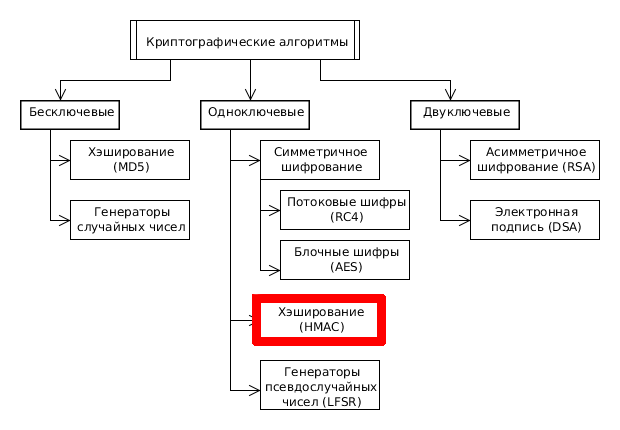
\includegraphics[width=\linewidth]{./images/png/CA_classification_hash.png}

\end{frame}

\begin{frame}
  \frametitle{Описание проблемы}

  \begin{itemize}
    \item{Как Боб может быть уверенным, что сообщение в самом деле пришло от Алисы?}
    \item{Канал передачи сообщений зачастую является небезопасным (интернет)}
    \item{Злоумышленник может не только перехватывать сообщения, но также изменять их или создавать новые}
  \end{itemize}
\end{frame}

\begin{frame}
  \frametitle{Возможное решение}

  \begin{itemize}
    \item{Алиса может добавлять ``подпись`` к сообщению, тем самым подтверждая авторство сообщения}
    \item{Боб должен иметь возможность проверить ``подпись`` Алисы}
    \item{``Подпись`` Алисы не может быть подделана злоумышленником}
  \end{itemize}
\end{frame}

\begin{frame}
  \frametitle{MAC (message authentication code)}

  \textbf{Цель}: обеспечение целостности сообщения и аутентификация источника данных.
  
  \vspace{1em}

  \begin{block}{Примеры:}
    \begin{itemize}
      \item{Защита файлов на диске от изменений}
      \item{Защита от изменения передаваемых по сети данных}
    \end{itemize}
  \end{block}

\end{frame}


\begin{frame}
  \frametitle{MAC (message authentication code)}

  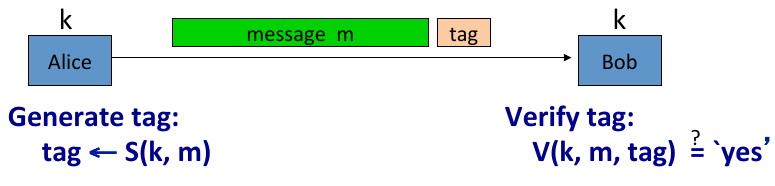
\includegraphics[width=\linewidth]{./images/png/MAC_protocol.png}

  \define{\textbf{MAC} (Имитовставка)} {пара алгоритмов $I=(S, V)$, определенных на $(K,M,T)$:
    \[ S(k,m) \rightarrow t \in T \]
    \[ V(k,m,t) \rightarrow \set{yes, no} \]
  }
  
\end{frame}


\begin{frame}
  \frametitle{MAC (message authentication code)}

  \begin{itemize}
    \item{Для обеспечения аутентификации при построении MAC должен быть использован секретный ключ}
    \item{В противном случае злоумышленник может изменить содержимое сообщения и построить для измененного сообщения MAC}
  \end{itemize}

\end{frame}


\begin{frame}
  \frametitle{Безопасность MAC}

  \begin{block}{Возможности злоумышленника}
    Значения MAC для выбранных злоумышленником сообщений $m_{1},m_{2},\ldots,m_{q}$ 
     ($t_{i} \leftarrow S(k,m_{i})$)
  \end{block}

  \begin{block}{Цель злоумышленника}
    Фальсификация данных:
    необходимо найти \textbf{новую} допустимую пару сообщение/тэг
    $(m,t) \notin \set{(m_{1}, t_{1}),\ldots,(m_{q}, t_{q})}$
  \end{block}

  \begin{block}{MAC --- безопасный, если:}
    \begin{itemize}
      \item{Злоумышленник не может найти допустимый тэг для нового сообщения $m$}
      \item{Злоумышленник не может найти новый допустимый тэг $(m, t')$, зная пару $(m,t)$}
    \end{itemize}
  \end{block}
  
\end{frame}


\begin{frame}
  \frametitle{Пример использования MAC}

  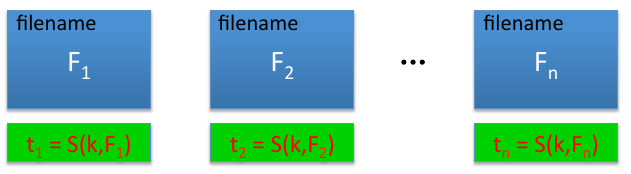
\includegraphics[width=\linewidth]{./images/png/MAC_example_FS.png}
  
  \begin{itemize}
    \item{При установке ОС считает MAC для всех системных файлов, используя в качестве
      ключа значение, полученное на основе пароля администратора. MAC дописывается в конец файла}
    \item{Позже вирус заражает некоторые системные файлы}
    \item{Администратор может обнаружить зараженные файлы, проверив MAC}
  \end{itemize}
\end{frame}


\begin{frame}
  \frametitle{Безопасная PRF - безопасный MAC}

  Для PRF $F: K \times X \rightarrow Y$ можно определить MAC $I_{F}=(S,V)$:

  \begin{itemize}
    \item{$S(k,m) := F(k,m)$}
    \item{$V(k,m,t) = \left\{
        \begin{array}{l} 
          yes, t=F(k,m) \\
          no, t \neq F(k,m)
        \end{array}
      \right.$}
  \end{itemize}

  \theorema{Если $F: K \times X \rightarrow Y$ --- безопасная PRF и 
    величина $1/|Y|$ пренебрежительно малa, то $I_{F}$ --- безопасный MAC}

\end{frame}


\begin{frame}
  \frametitle{Получение безопасного MAC из PRF}

  \begin{itemize}
    \item{AES: MAC для 128-битных сообщений}
    \item{Возможно ли получить MAC для больших сообщений, используя MAC для маленьких сообщений?}
    \item{На практике используются два алгоритма:
      \begin{itemize}
        \item{CBC-MAC (стандарт в финансовых приложениях)}
        \item{HMAC (интернет протоколы: SSL, IPSec, SSH)}
      \end{itemize}
    }
    \item{Оба протокола преобразуют MAC для маленьких сообщений в МАС для больших сообщений}
  \end{itemize}
\end{frame}


\begin{frame}
  \frametitle{Encrypted CBC-MAC}

  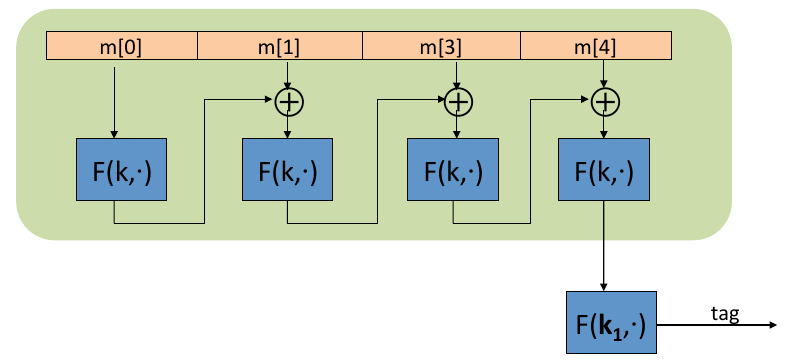
\includegraphics[width=\linewidth]{./images/png/ECBC_MAC.png}

  $F:K \times X \rightarrow X$ - псевдослучайная перестановка (PRP)
  $F_{ECBC}:K^{2} \times X^{\le L} \rightarrow X$ - псевдослучайная функция (PRF)

\end{frame}

\begin{frame}
  \frametitle{Атака расширения на ECBC-MAC}

  \begin{block}{Expansion attack}
    \begin{itemize}
      \item{Выбрать случайное сообщение $m \in X$ из одного блока}
      \item{Запросить значение тега для $m$. $t=F(k,m)$}
      \item{Выдать $t$ как как тег для нового двублочного сообщения $m1 = (m, t \oplus m)$}
    \end{itemize}
  \end{block}
\end{frame}

\begin{frame}
  \frametitle{Дополнение блоков данных (padding)}

  \begin{itemize}
    \item{Что делать, если длина сообщения не кратна размеру блока?}
    \item{Плохая идея: добить последний блок нулями}
    \item{Функция дополнения блока данных должна быть обратимой $m_0 \neq m_1 \rightarrow pad(m_0) \neq pad(m_1)$}
    \item{Простое решение: добавлять ``100...0``}
    \item{Необходимо добавлять фиктивный блок, если длина сообщения кратна размеру блока}
  \end{itemize}
\end{frame}

\begin{frame}
  \frametitle{Алгоритм CMAC (стандарт NIST)}

  \begin{itemize}
    \item{Вариант CBC-MAC}
    \item{Использует 3 ключа: $k$, $k_1$, $k_2$}
    \item{Нет необходимости в заключительном шаге шифрования дополнительным ключом}
    \item{Нет необходимости добавлять фиктивный блок}
  \end{itemize}

  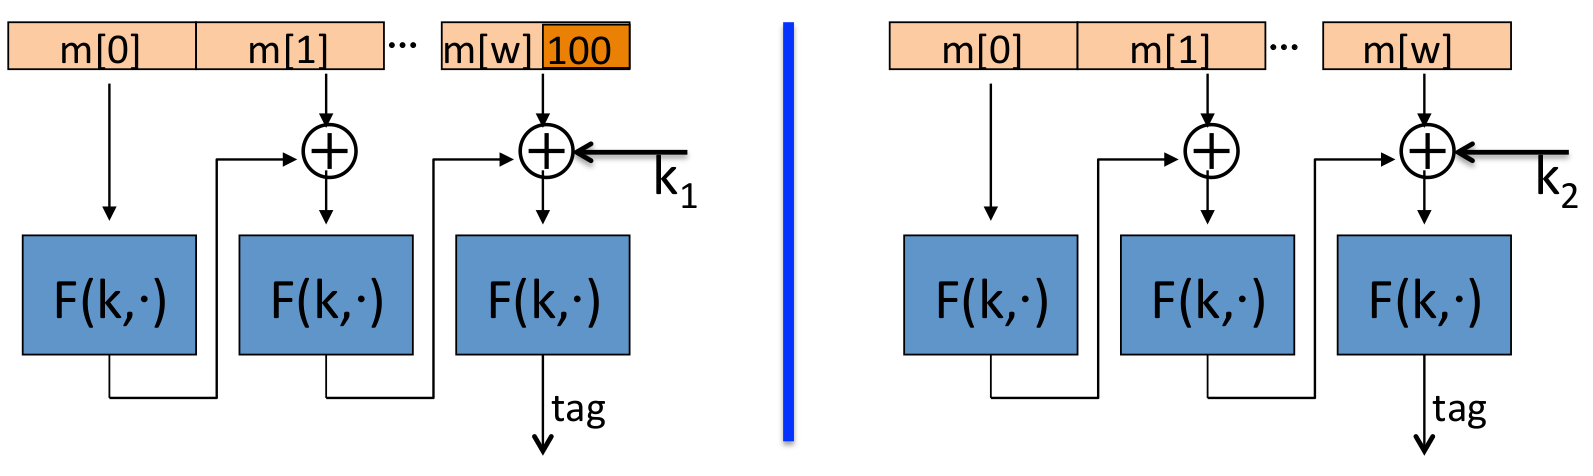
\includegraphics[width=\linewidth]{./images/png/CMAC.png}

\end{frame}

\begin{frame}
  \frametitle{Parallel MAC}

  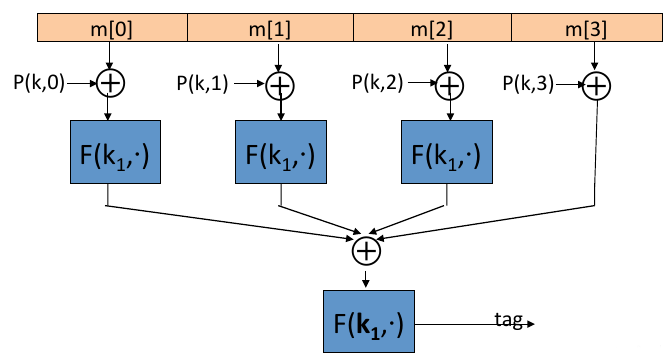
\includegraphics[width=\linewidth]{./images/png/PMAC.png}

  %$F:K \times X \rightarrow X$ - псевдослучайная перестановка (PRP)
  $F_{PMAC}:K^{2} \times X^{\le L} \rightarrow X$ - псевдослучайная функция (PRF)

  \begin{block}{Преимущества}
    \begin{itemize}
      \item{Возможна параллельная реализация}
      \item{Инкрементальное обновление}
    \end{itemize}
  \end{block}
\end{frame}

\end{document}
